\subsection{Progettazione architetturale}
Il periodo di \textit{Progettazione architetturale} comincia il giorno dopo la presentazione per la \textit{Revisione dei requisiti} (22/01/2019) e si conclude con la consegna dei documenti per la \textit{Revisione di Progettazione} (08/03/2019). Le attività principali sono:
\begin{itemize}
	\item\textbf{Incremento e verifica:} all'inizio del periodo vengono svolte attività di incremento e verifica sui vari documenti consegnati alla \textit{Revisione dei requisiti}
	\item\textbf{Glossario:} questa attività comprende sia il miglioramento del Glossario che l’aggiunta di nuovi termini;
	\item\textbf{Manuale Utente:}  questa attività consiste nella redazione del Manuale Utente, contenente indicazioni sull’utilizzo del programma che sta venendo prodotto;
	\item\textbf{Definizione di prodotto:} questa attività consiste nella redazione del documento della Definizione di Prodotto contenente i dettagli della progettazione architetturale;
	\item\textbf{Lettera di presentazione:} Lettera di presentazione: questa attività prevede la stesura della Lettera di presentazione per la \textit{Revisione di Progettazione};
	\item\textbf{Baseline Tecnologica:} questa attività consiste nella redazione da parte dei Progettisti del documento della \textit{Tecnology Baseline}\ped g, contenente le scelte progettuali ad alto livello, le tecnologie e i framework utilizzati;
	\item \textbf{Proof of Concept:} Realizzazione di un piccolo prototipo del Plugin da realizzare.
\end{itemize}

\begin{figure}[h!]
	\centering
	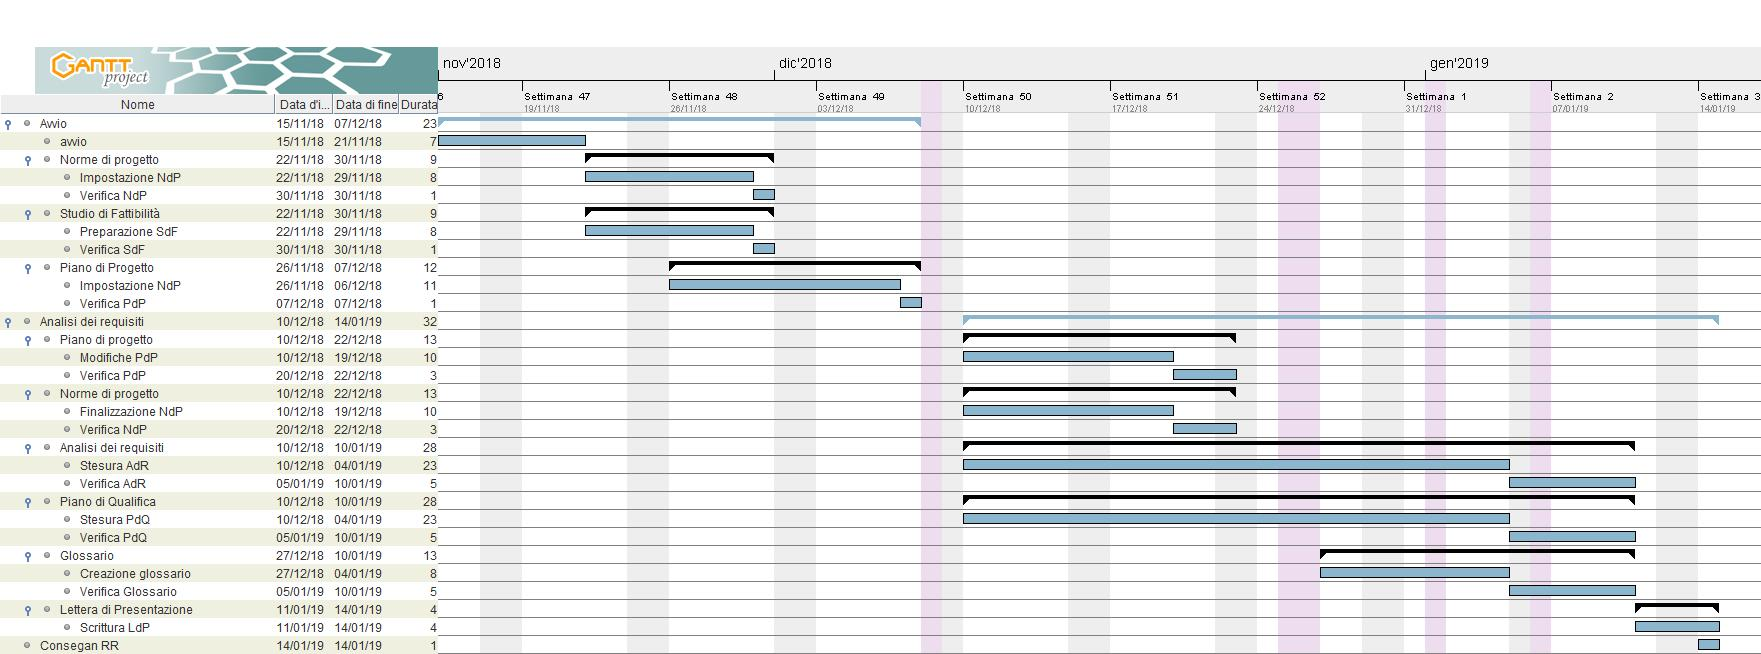
\includegraphics[width=\textwidth]{Gantt_seconda_fase.jpg}
	\caption{Diagramma di Gantt per la fase fino alla Revisione di Progettazione}
\end{figure}

\begin{figure}[h!]
	\centering
	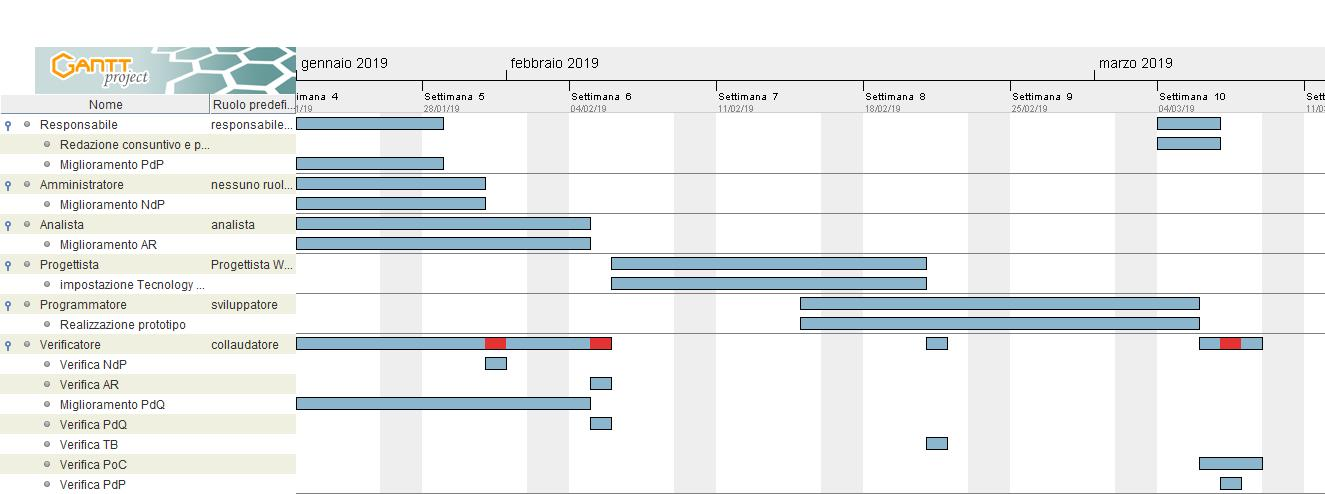
\includegraphics[width=\textwidth]{Gantt_seconda_fase_risorse.jpg}
	\caption{Diagramma di Gantt delle risorse fino alla Revisione di Progettazione}
\end{figure}

\begin{table}[h!]
	\centering
	\renewcommand{\arraystretch}{1.5}
	\begin{tabular}{|l|p{4.5cm}|p{4.5cm}|}
		\hline
		\multicolumn{3}{|c|}{\textbf{Suddivisione temporale}}\\
		\hline
		\textbf{Ruolo} & \textbf{22/01/19 - 13/02/19} & \textbf{13/2/19 - 08/03/2019} \\
		\hline
		\textbf{Responsabile} & \daL & \daG \\
		\hline
		\textbf{Amministratore} & \daG & \gia \\
		\hline
		\textbf{Analista} & \parbox{4.5cm}{\pie\\ \mic\\ \mar\\ \gia} & - \\
		\hline
		\textbf{Progettista} & \mat &  \parbox{4.5cm}{\daL \\ \mar} \\
		\hline
		\textbf{Programmatore} & - & \mic \\
		\hline
		\textbf{Verificatore} & - &  \parbox{4.5cm}{\mat \\ \pie} \\
		\hline
	\end{tabular}
	\caption{suddivisione temporale della Progettazione architetturale}
\end{table}